\documentclass{article} 
\usepackage{polyglossia} 
\usepackage{amsmath}
\usepackage{fontspec} 
\usepackage{lipsum} 
\usepackage[margin=1in]{geometry}
\usepackage{graphicx} 
\usepackage{caption} 
\usepackage{subcaption}
\usepackage{hyperref} 
\usepackage{listing}
\hypersetup{% 
    colorlinks=true, linkcolor=blue, filecolor=magenta,      
    urlcolor=cyan, 
    pdfinfo = {%
        Title = Αναφορά 2ης Εργασίας ΨΕΕ
        Author = {Χρήστος Μάριος Περδίκης},
        Producer = XeLaTeX,
    } 
}

\setmainfont{C059}

\title{Ψηφιακή Επεξεργασία Εικόνας \\ Ανίχνευση Ακμών και Κύκλων}
\date{Εαρινό Εξάμηνο 2024-2025}
\author{Χρήστος-Μάριος Περδίκης 10075 cperdikis@ece.auth.gr}

\begin{document}
\maketitle

%Τι πρέπει να αλλάξω; 
%circ_hough.py:
%Έξοδος όλων των κύκλων που έχουν ψήφους πάνω από το V_min.
 
Αυτή είναι η αναφορά για την 2η εργασία του μαθήματος Ψηφιακή Επεξεργασία 
Εικόνας. Ο στόχος της εργασίας είναι η ανίχνευση ακμών με τους τελεστές Sobel
και Laplacian of Gaussian και η ανίχνευση κύκλων με βάση τον αλγόριθμο Hough.
Ακολουθεί η επεξήγηση του demo.py και των παραδοτέων συναρτή\-σεων.

\section{Αρχείο επίδειξης demo.py}
Στο αρχείο demo.py καλούνται όλες οι παραδοτέες συναρτήσεις για να γίνει η 
μελέτη πάνω στην εικόνα της εκφώνησης. Πρώτα φορτώνεται η εικόνα και μετά 
σμικρύνεται στο ένα δέκατο της αρχικής της ανάλυσης. Αυτό γίνεται για την βελτίωση
της απόδοσης του κώδικα, η εκτέλεση του αλγόριθμου Hough παίρνει πολύ ώρα για την
αρχική ανάλυση. Για αυτές τις λειτουργίες χρησιμοποιήθηκε η βιβλιοθήκη
opencv. Η αρχική και η σμικρυσμένη εικόνα εμφανίζονται στην οθόνη 
(εικόνα~\ref{origin_shrunk}) με αναμενόμενο 
αποτέλεσμα να φαίνονται ολόιδιες. Για την προβολή των εικόνων 
χρησιμοποιήθηκε η βιβλιοθήκη matplotlib. Έπειτα καλείται η συνάρτηση  sobel\_edge 
για ανίχνευση ακμών 
με τελεστή Sobel πέντε φορές μια για κάθε κατώφλι $thresholds = \left[50,100,150,
200,250\right]$. Η επεξήγηση της συνάρτησης sobel\_edge βρίσκεται στην 
ενότητα~\ref{sobel}. Η δυαδική εικόνα με $threshold = 150$ αποθηκεύεται για μετέπειτα
χρήση ως είσοδος στον αλγόριθμο Hough. Καλείται η συνάρτηση log\_edge μία φορά 
για την ανίχνευση ακμών με
τελεστή Laplacian of Gaussian. Η επεξήγηση της συνάρτησης sobel\_edge βρίσκεται στην 
ενότητα~\ref{log}. Οι δυαδικές εικόνες-αποτελέσματα των δύο συναρτήσεων 
προβάλλονται στην οθόνη μαζί και δίπλα τους δημιουργείται
ένα plot του αριθμού των σημείων ακμών που βρέθηκαν για διάφορες τιμές κατωφλίων
για τον αλγόριθμο sobel (εικόνα~\ref{lognsobel}). 

Από τα αποτελέσματα των αλγορίθων εύρεσης ακμών με τελεστές Sobel και LoG 
μπορούμε να εξάγουμε τα εξής συμπεράσματα. 
Μεταξύ των δυαδικών εικόνων Sobel βλέπουμε ότι όσο μικρότερο είναι το κατώφλι,
τόσο έντονες φαίνονται οι ακμές της εικόνας. Για πολύ μικρές τιμές 
π.χ. για $threshold = 50$ εμφανίζεται θόρυβος ο οποίος είναι ανεπιθύμητος, δεν 
αντιστοιχεί σε ακμές. Συγκρίνοντας τις εικόνες Sobel με την εικόνα LoG βλέπουμε
ότι η δεύτερη έχει περισσότερο θόρυβο από τις εικόνες 
Sobel. Αυτό είναι αναμενόμενο, καθώς από τη φύση του η μέθοδος του τελεστή LoG
είναι πιο ευαίσθητη στον θόρυβο, με το αντάλλαγμα ότι μπορεί να ανιχνεύει πιο 
λεπτές ακμές. Στην παρούσα εφαρμογή φαίνεται ο τελεστής Sobel να κάνει καλύτερη
δουλειά, αν και οι δύο μέθοδοι ανιχνεύουν επιτυχώς τις κύριες ακμές τις εικόνας.

Ακολουθεί η ανίχνευση κύκλων με Hough. Ο αλγόριθμος Hough εκτελέστηκε και για
δυαδική εικόνα Sobel για $threshold = 150$ και για την δυαδική εικόνα LoG. 
Η δυαδική εικόνα αυτή είναι η είσοδος της συνάρτησης circ\_hough. 
Η υλοποίηση του αλγορίθμου Hough για κύκλους επεξηγείται αναλυτικά στην 
ενότητα~\ref{hough}. 
Αρχικοποιούνται οι διαστάσεις του πίνακα Hough (32 για τετμημένη και τεταγμένη
του κέντρου του πιθανού κύκλου και 32 για την ακτίνα του κύκλου), η μέγιστη 
ακτίνα του κύκλου στο μισό της μικρότερης διάστασης της εικόνας και οι ελάχιστες
ψήφοι για να ανιχνευτεί ο κύκλος. Υπάρχουν δύο πίνακες $V_{min}$:
\begin{itemize}
    \item Sobel: $V_{min} = \left[500, 750, 1000\right]$
    \item LoG: $V_{min} = \left[600, 800, 1000\right]$
\end{itemize}
Ο αλγόριθμος τρέχει για κάθε μία από τις τιμές κατωφλίου.

Εφόσον ανιχνευτεί κύκλος, αυτός ζωγραφίζεται πάνω από την αρχική εικόνα 
(τη σμικρυσμένη ασπρόμαυρη εικόνα που φορτώθηκε στην αρχή, όχι τη δυαδική εικόνα). 
Τα αποτελέσματα του Hough για όλες τις τιμές κατωφλίου ψήφων και τις δύο διαφορετικές
εικόνες εισόδου προβάλλονται όλα στην οθόνη (εικόνα~\ref{}). Μπορούμε να εξάγουμε
το συμπέρασμα ότι η τιμή του κατωφλίου $V_{min}$ είναι πολύ σημαντική για τον
επιτυχή εντοπισμό του κύκλου. Για χαμηλή τιμή κατωφλίου υπάρχουν πολλά false positives,
ενώ για πολύ μεγάλη τιμή του κατωφλίου δεν ανιχνεύεται κανένας κύκλος. Δεν υπάρχουν
μεγάλες διαφορές μετξαύ των διαφορετικών εικόνων Sobel και LoG. Υπάρχουν μερικά
false positives που είναι διαφορετικά και ο πλειοψηφικός κύκλος είναι λίγο εκτοπισμένος
για εικόνα εισόδου LoG, αλλά οι διαφορές είναι αμελητέες. Τα αποτελέσματα φαίνονται στην
εικόνα~\ref{sobel_hough}.

\section{fir\_conv}
Η συνάρτηση fir\_conv υλοποιεί δισδιάστατη συνέλιξη μεταξύ μιας grayscale
εικόνας και ενός FIR φίλτρου / πεπερασμένης συνελικτικής μάσκας. Βρίσκεται στο 
αρχείο fir\_conv.py. Έχει προαιρετική είσοδο τις αρχές των συντεταγμένων 
της εικόνας και της συνελικτικής μάσκας. Αν δεν δοθεί η προαιρετική είσοδος, η αρχή 
των συντεταγμένων για τη συνελικτική μάσκα είναι το κέντρο της. Για την εικόνα
η αρχή των συντεταγμένων της είναι αυτή που ορίστηκε όταν φορτώθηκε σε numpy 
array από την συνάρτηση imread της opencv, δηλαδή η πάνω αριστερά γωνία.
Υπολογίζονται οι διαστάσεις της εικόνας εξόδου της συνέλιξης.
Αν $N_1$ και $N_2$ οι διαστάσεις της εικόνας και $n_1$ και $n_2$ οι διαστάσεις
της μάσκας, η εικόνα εξόδου θα έχει διαστάσεις $(N_1 - n_1 + 1, N_2 - n_2 + 1)$.
Η αρχή των συντεταγμένων της εικόνας εξόδου είναι το άθροισμα της αρχής των συντεταγμένων της 
εικόνας με την αρχή των συντεταγμένων της συνελικτικής μάσκας. Η συνέλιξη 
πραγματοποιείται ολισθαίνοντας την συνελικτική μάσκα πάνω από την εικόνα εισόδου
και αθροίζοντας τα γινόμενα των στοιχείων της μάσκας με τα αντίτοιχα στοιχεία 
της εικόνας. Η εικόνα εξόδου είναι το αποτέλεσμα της συνέλιξης και η αρχή των 
συντεταγμένων αυτής της εικόνας.

\section{sobel\_edge}\label{sobel}
Η συνάρτηση sobel\_edge υλοποιεί την μέθοδο εύρεσης ακμών με τον τελεστή 
Sobel. Βρίσκεται στο αρχείο sobel\_edge.py. Βρίσκει τις ακμές μιας εικόνας
εισόδου και παράγει ως έξοδο μια δυαδική εικόνα που έχει άσπρα pixels στις 
ακμές και μαύρα pixels οπουδήποτε αλλού. Αρχικά ορίζονται οι δύο μάσκες Sobel
για την τεταγμένη και την τετμημένη:

\begin{gather}
    sobel_x = \left[\begin{matrix}
        -1& 0& 1 \\
        -2& 0& 2 \\
        -1& 0& 1
    \end{matrix}\right] \\
    sobel_y = \left[\begin{matrix}
        -1& -2& -1 \\
         0&  0&  0 \\
         1&  2&  1
    \end{matrix}\right] 
\end{gather}
Έπειτα χρησιμοποιείται η συνάρτηση fir\_conv για να συνελιχθεί οι $sobel_x$ και
$sobel_y$ με την εικόνα. Με αυτόν τον τρόπο υπολογίζεται το gradient της αρχικής
εικόνας κατά άξονα $x$ και $y$ αντίστοιχα ($grad_x$, $grad_y$). Έπειτα υπολογίζεται 
το μέτρο του συνολικού gradient για κάθε σημείο:

\begin{equation}
    |gradient| = \sqrt{grad_x^2 + grad_y^2}
\end{equation}
Δημιουργείται μια νέα εικόνα ίδιων διαστάσεων με την εικόνα εισόδου στην οποία 
τα pixels που έχουν $|gradient| \geq threshold$ βάφονται άσπρα και όλα τα 
υπόλοιπα βάφονται μαύρα. Αυτή είναι η δυαδική εικόνα εξόδου.

\section{log\_edge}\label{log}
H συνάρτηση log\_edge υλοποιεί τη μέθοδο εύρεσης ακμών με τον τελεστή
Laplacian of Gaussian. Βρίσκεται στο αρχείο log\_edge.py. Όμοια με τη 
μέθοδο sobel\_edge, βρίσκει τις ακμές της εικόνας εισόδου και 
παράγει μια δυαδική εικόνα εξόδου με άσπρα pixels στις θέσεις των ακμών
της αρχικής εικόνας και μαύρα pixels οπουδήποτε αλλού. Αρχικά ορίζεται 
ο πίνακας συντελεστών LoG:

\begin{equation}
h = \left[\begin{matrix}
        0& 0&-1& 0& 0 \\
        0&-1&-2&-1& 0 \\
       -1&-2&16&-2&-1 \\
        0&-1&-2&-1& 0 \\
        0& 0&-1& 0& 0 
    \end{matrix}\right]
\end{equation}
και κανονικοποιείται έτσι ώστε να λαμβάνει τιμές στο διάστημα $\left[0,1\right]$.
Με τη χρήση της συνάρτησης fir\_conv πραγματοποείται σνέλιξη μεταξύ του πίνακα
$h$ και της εικόνας εισόδου. Για να βρεθούν τα σημεία στα οποία υπάρχουν zero 
crossings, γίνεται έλεγχος για κάθε pixel της προκύπτουσας εικόνας. Αν αυτό έχει 
διαφορετικό πρόσημο από οποιοδήποτε pixel-γείτονα προς 8 κατευθύνσεις και η 
παράγωγος της προκύπτουσας εικόνας σε αυτό το
pixel είναι πάνω από ένα όριο, τότε σε αυτό το σημείο υπάρχει zero-crossing και 
θεωρείται σημείο ακμής. Για το όριο επιλέχθηκε η σταθερά 10, πειραματικά παρατηρήθηκε
ότι ήταν μια ικανοποιητική τιμή. Όμοια με τον τελεστή Sobel, δημιουργείται μια δυαδική 
εικόνα εξόδου με άσπρα pixels στις θέσεις των ακμών της αρχικής εικόνας και μαύρα 
pixels οπουδήποτε αλλού. Το μέτρο της παραγώγου σε κάθε pixel 
είναι η ρίζα του αθροίσματος των τετραγώνων των παραγώγων της εικόνας προς τους 
δύο άξονες (όμοια διαδικασία με τον τελεστή Sobel). Οι παράγωγοι υπολογίστηκαν 
χρησιμοποιώντας την προσέγγιση των κεντρικών διαφορών.

\section{circ\_hough}\label{hough}
Σε αυτή τη συνάρτηση τροποποιείται ο αλγόριθμος Hough για ευθείες 
έτσι ώστε να ανιχνεύει κύκλους. Βρίσκεται στο αρχείο circ\_hough.py.
Λαμβάνει ως είσοδο μια δυαδική εικόνα ακμών, τη μέγιστη ακτίνα 
που μπορεί να έχει ο πιθανός κύκλος, τις διαστάσεις του πίνακα Hough, δηλαδή
τις διαστάσεις για την διακριτοποίηση, και τον αριθμό των ελαχίστων 
ψήφων που χρειάζονται για να ανιχνευτεί κύκλος. Αρχι\-κο\-ποι\-είται ο 
3D πίνακας ψηφοφορίας Hough με τις διαστάσεις που ορίζει η είσοδος $dim$
και υπολογίζονται οι τιμές steps που χρειάζεται για να προσπελαστεί το επόμενο
bin για κάθε διάσταση. Για κάθε pixel ακμής $(x, y)$ ερευνάται ποιοί κύκλοι με
κέντρο $(a, b)$ και ακτίνα $r$ περνάνε από τα $(x, y)$. Για κάθε τριπλέτα 
κύκλου $(a, b, r)$ για την οποία ισχύει η προηγούμενη πρόταση, προστίθεται
μία ψήφος στην αντίστοιχη θέση του πίνακα ψηφοφορίας Hough. Ο
υπολογισμός του γεωμετρικού τόπου γίνεται με την εξίσωση του κύκλου σε
καρτεσιανές συντεταγμένες:

\begin{equation}\label{circ_eq}
    (a - x)^2 + (b - y)^2 = r^2
\end{equation}
όμως λόγω διακριτοποίησης υπάρχει περίπτωση να υπάρχουν σφάλματα ακριβείας, για
αυτό η~\ref{circ_eq} τροποποι\-είται ώστε να ικανοποιείται με ένα κατώφλι:

\begin{equation}\label{circ_eq2}
    \sqrt{(a - x)^2 + (b - y)^2} - r < tolerance 
\end{equation}
όπου $tolerance = max(0.01, 0.1*r)$. Οι τριπλέτες $(a, b, r)$ που έχουν 
στον πίνακα Hough περισσότερες ψήφους από την τιμή της $V_{min}$ προστίθονται σε μία λίστα.
Αυτή μετατρέπεται σε numpy array και είναι η έξοδος της συνάρτησης. Αν
δεν υπάρχει κύκλος που να έχει πάνω από $V_{min}$ ψήφους, η συνάρτηση 
επιστρέφει άδεια arrays, με τη λογική ότι δεν ανιχνεύθηκε κύκλος. Θα μπορούσαμε 
σε αυτήν την περίπτωση αντί για άδεια arrays να επιστρέφαμε τον κύκλο με τις 
περισσότερες ψήφους. Ο κώδικας για αυτήν την προσέγγιση είναι commented στο 
αρχείο circ\_hough.py στις γραμμές 65-75, αν γίνει uncommented τότε το πρόγραμμα
θα δουλέψει με αυτόν τον εναλλακτικό τρόπο. Η συνάρτηση κάνει print το πόσους
κύκλους επιστρέφει σε κάθε κλήση της και, αν δεν επιστρέψει κανέναν κύκλο,
τον μέγιστο αριθμό ψήφων που μετρήθηκε. Αυτοί οι αριθμοί βοηθούν στην 
κατάλληλη τροποποίηση των κατωφλίων $V_{min}$.


\section{Αποτελέσματα σε Εικόνες}

\begin{figure}
    \centering
    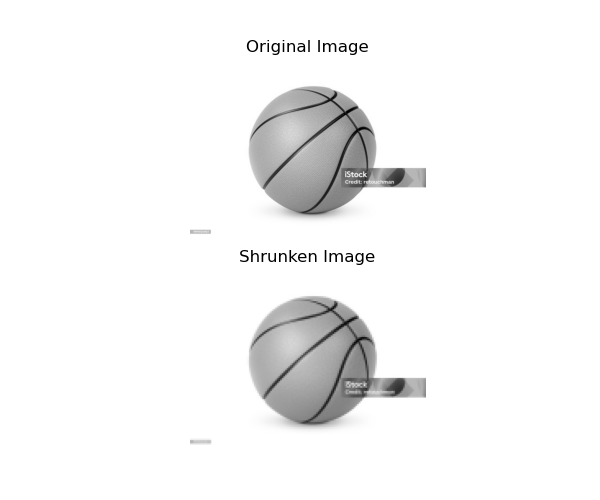
\includegraphics[width=\textwidth]{origin_shrunk.png}
    \caption{Η αρχική εικόνα και η σμικρυσμένη εκδοχή της}\label{origin_shrunk}
\end{figure}

\begin{figure}
    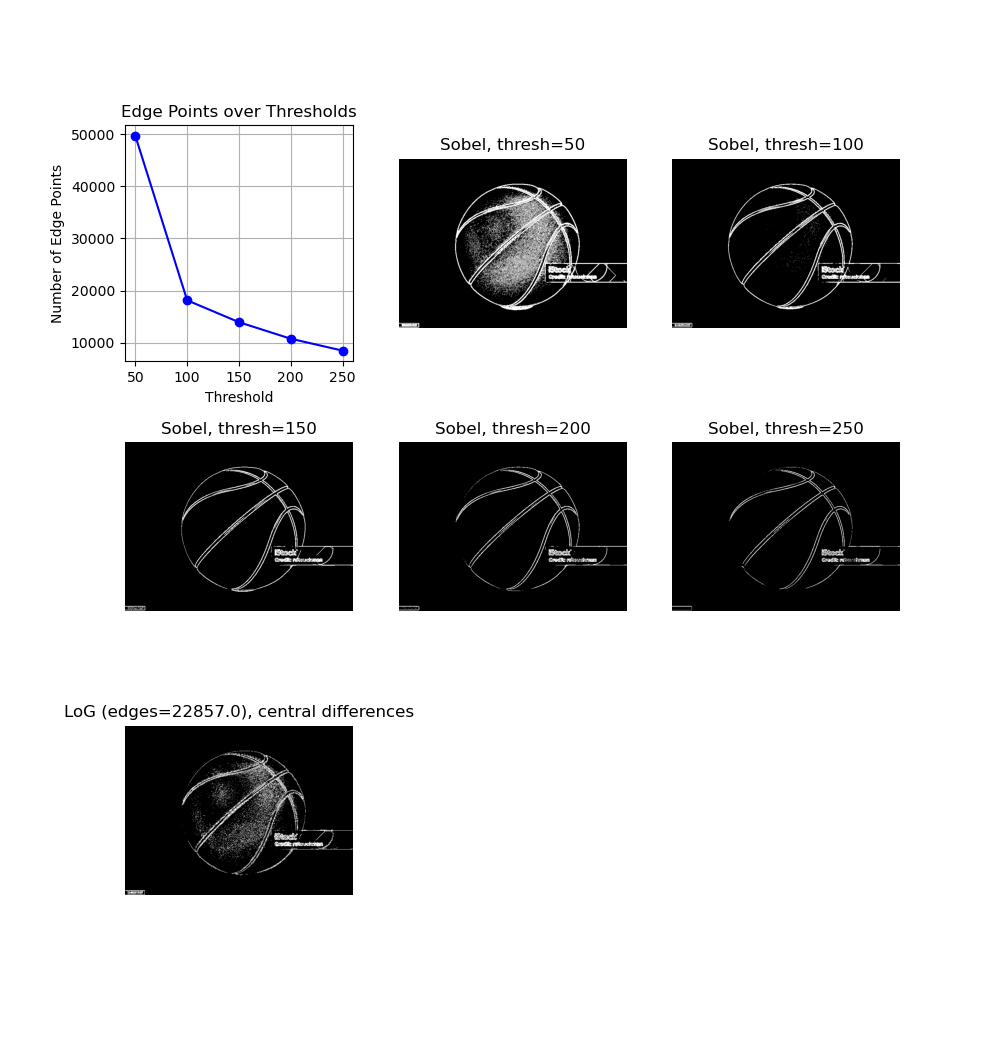
\includegraphics[width=\textwidth]{log_n_sobel.png}
    \caption{Δυαδικές εικόνες από ανίχνευση ακμών με Sobel και LoG. Γράφημα αριθμού
    σημείων ακμών προς τιμών threshold για ανίχνευση ακμών με Sobel.}\label{lognsobel}
\end{figure}

\begin{figure}
    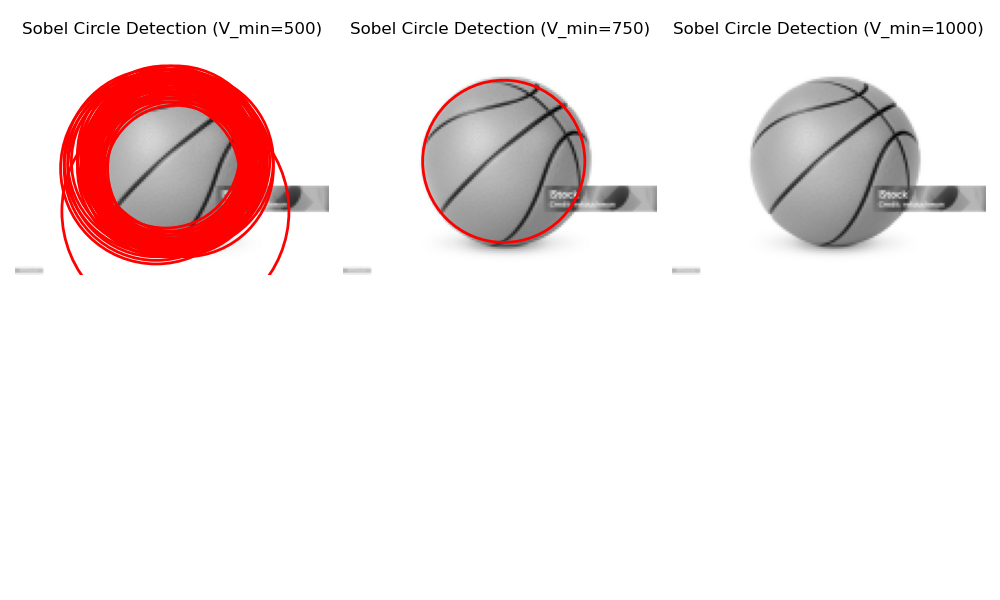
\includegraphics[width=\textwidth]{sobel_circle.png}
    \caption{Αποτέλεσμα αλγόριθμου Hough για είσοδο δυαδική εικόνα ακμών τελεστή Sobel}\label{sobel_hough}
\end{figure}

\begin{figure}
    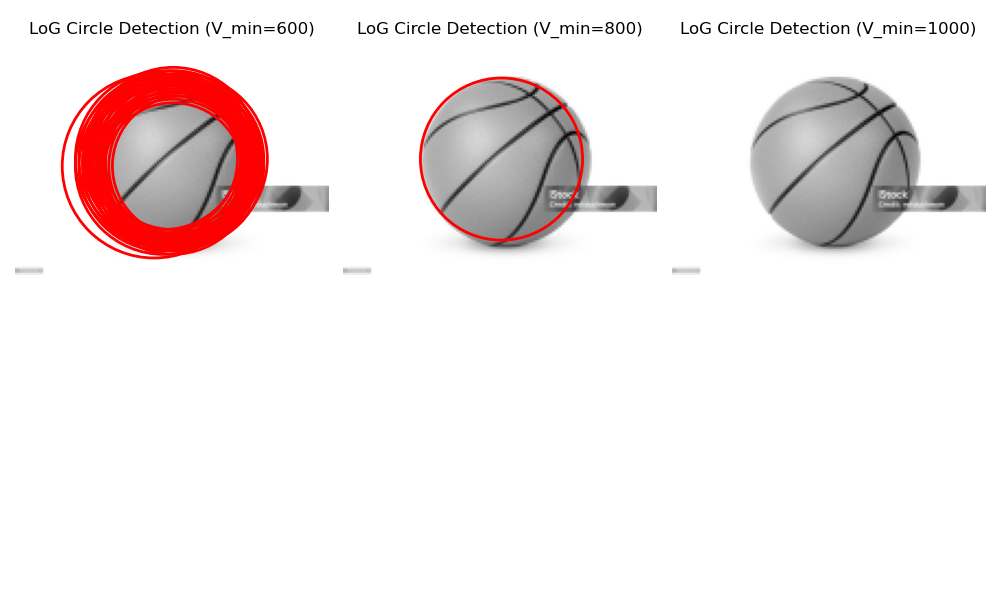
\includegraphics[width=\textwidth]{log_circle.png}
    \caption{Αποτέλεσμα αλγόριθμου Hough για είσοδο δυαδική εικόνα ακμών τελεστή LoG}\label{sobel_hough}
\end{figure}

\end{document}
